

\section{Service Scope}
Since the service is offered via the web it is accessible worldwide.  The service will be initially based in the UK.  The UK has good Internet connectivity on a worldwide scale, so is a fair location for the servers.  Future expansion plans may include setting up mirrors of the service in other geographical locations to better service those areas.

\section{Description of Customers}
There will be two main categories of customer: developers and novice users.  They will have slightly different uses for the service. 

\subsection{Developers}
Developers are the people that create the software.  There can be a few or as many as hundreds or thousands of developers working on a project and they use the mailing lists to co-ordinate the work they are doing on the software.   Developers will be using the service to keep track of developments of the projects they are working on.  They may want to look back at previous discussions and keep a peripheral view on the discussions happening on a related project without flooding their mailbox with email.

\subsection{Novice Users}
With the rise in popularity of alternative operating systems such as Linux, more and more novice users are entering the realm of what has traditionally been considered the domain of experienced users only.  Although it is growing there is currently not very much printed documentation for these operating systems and applications -- this is mainly due to the rapid development pace of these projects.  Consequently often the best place for new users to look for information is on the mailing lists.  If a user is just looking for the answer to what is probably a common question, they probably do not want to subscribe to the mailing list just to find out the answer.  Also they are unlikely to get a response to their question if it was just asked last week by someone else.


To start with we will be concentrating on the Developers rather than the Novice users.  This is simply because the Developers will be looking for a simple clean system that just does the job.  The novice users will want more features to help them navigate the vast amounts of data.  We could also provide extra services such as collections of other documentation and FAQs \footnote{Frequently Asked Questions}.

\section{Customer Needs and Benefits}
\label{sec:survey}{}
There are several main needs of the customers:

\begin{itemize}
\item To be able to search for answers to questions
\item To keep in touch with what is happening on lists
\item To use the site as a replacement for reading mailing list messages in their mailbox.
\end{itemize}

This was found by a survey that was filled in by 50 participants.  The survey was 10 short questions about the mailing list usage of the participant.  The results were more from the developers than the novice users as they were the easiest to get ahold of and the most willing to fill in the survey.  

The survey was announced on a couple of Internet news forums and most of the participants filled in the survey within 6 hours of it being announced.  From the web server log files it can be seen that 126 people visited the survey page

\begin{figure}[!ht]
\begin{center}
\begin{tabular}{cc}
\epsfig{file=survey/lists.eps,height=4.5cm}
&
\epsfig{file=survey/posts.eps,height=4.5cm}
\end{tabular}
\end{center}
\caption{Survey Results}
\end{figure}

The results of the survey were very promising.  Over half the recipients that responded indicated that they are subscribed to over 5 lists, showing that indeed the lists are used a lot.

Most people send less than 10 messages a week to the lists. This shows that the emphasis is on reading messages rather than writing them -- obviously if everybody wrote as many messages as they read chaos would ensue!  However, nearly a third of the respondents send zero messages a week, these people are prime customers.  They are only observers on the lists and would probably welcome a less intrusive way of reading all the messages, than subscribe to each list.


\begin{figure}[!ht]
\begin{center}
\begin{tabular}{cc}
\epsfig{file=survey/freq.eps,height=4.5cm}
&
\epsfig{file=survey/where.eps,height=4.5cm}
\end{tabular}
\end{center}
\caption{Survey Results}
\end{figure}

The survey also asked how often people use existing archive services for the lists -- either to read or to search for messages.  The majority of respondents indicated that they used the archives once a week.  This shows that we should expect a large number of regular repeat visitors.

Many Open Source projects keep their own mailing list archives on their site, however as noted earlier their searching facilities are generally primitive and archives are not updated as often as one would like.  These sites are still the most popular place for people to browse and search the archives.  This indicates that any other competitors out there have not made significant inroads into the market.  Dejanews is a site that the author uses quite frequently, which indexes newsgroups, not mailing lists, but even it does not seem to be very popular.

\begin{figure}[!ht]
\begin{center}
\epsfig{file=survey/rate.eps,height=4.5cm}
\caption{Survey Results}
\end{center}
\end{figure}

The participants were then asked to rate from 0 to 5, five aspects of an archive site as to how important they are.  The aspects were:

\begin{itemize}
\item Ability to Search
\item Ability to Browse
\item Ability to post messages to the lists
\item Customisability
\item Extra Features (eg. news, other documentation)
\end{itemize}

The results show that searching and browsing are the two most important aspects of the site, the other three all averaged right in the middle at 2.5.  Searching had an average score of 4.7 which was the highest, which confirms the need for good searching facilities on the site.

The results obtained from the survey are probably somewhat biased, in the fact that participants answered the survey voluntarily, and hence only those who have some interest in the mailing lists responded.  Once the site is up and running we hope to keep in close contact with the visitors by way of polls and surveys to make sure we spend our efforts effectively on developing the site in the right direction for all users.


\section{Market Size and Growth}
\subsection{Estimating the Market Size}
\label{sec:size}
As mentioned above more and more users are switching away from Microsoft Windows to alternative Operating Systems such as FreeBSD and Linux.  These are the biggest and most complex Open Source Projects and have the most numbers of mailing lists and subscribers.  Hence this is the area that most of this research has been done.

Estimating the market size of the different open-source user communities can be very difficult as there are no definitive surveys or studies.  Also since most can be freely downloaded and copied, we cannot simply ask a single vendor or source for figures.

A prediction was done to try and estimate the size of various communities in 1998.  This data is somewhat out of date now, but gives us an idea of what is now probably a minimum figure.  

The statistics were calculated by taking ratios of the number of posting to Internet newsgroups associated with each community, as measured by the Netscan analysis tool \footnote{Smith, Marc. 1997. "Netscan: A tool for measuring and mapping social cyberspaces" http://netscan.research.microsoft.com.}.  From the size of these groups the number of active users was extrapolated using a base of 7 million Linux users.


\begin{figure}[!ht]
\begin{center}
\epsfig{file=survey/percent.eps,width=6cm}
\end{center}
\end{figure}

\begin{center}
\begin{tabular}{|l|c|c|}
\hline
         & Number of Posters & Estimated Size of User Community \\
\hline
Linux    & 13,231  & 7,000,000  \\
Perl     & 2,023   & 1,000,000  \\
BSD      & 1,820   & 960,000    \\
Apache   & 738     & 400,000    \\
Sendmail & 670     & 350,000    \\
Python   & 612     & 325,000    \\
Tcl/tk   & 563     & 300,000    \\
Samba    & 309     & 160,000    \\
\hline
\end{tabular}
\end{center}

\subsection{Market Growth}

The latest figures show the Linux community to be around 12 - 14 million users \cite{www:lcp}. And studies show an astounding 40\% growth per year.

\section{Competitors}
There is currently only one direct competitor to OSDigger, that is GeoCrawler.  They also are targeting the Open Source community and have quite a large archive already.

\label{geocrawler}
\subsection{GeoCrawler}
GeoCrawler has 2,800,000 emails with 5,000 added each day.  This means it is roughly the same size the OSDigger will initially be.  It allows searching and browsing of the mailing lists and has some customization.  According to the web page the archive is created and updated by \emph{custom java spiders}.  This shows that they have been writing some software themselves, however the search software used is a public domain piece of software for searching web pages called \emph{HT://Dig}.  They only allow searches on a particular list, you cannot search across multiple lists.

They allow posting of messages to lists, which require users to apply for a free account and login before they do so.

From their web page they appear to be sponsored by Linux.com which is a large commercial Linux organization.

\subsection{MARC}
\textbf{M}ailing list \textbf{ARC}hive.  Was setup initially for internal use by a company, it then evolved into a public service.  Again, to search you have to specify a particular list and a particular year first.  The data is stored in the same database, mySQL, that OSDigger uses.  It allows customization of colour scheme, but not much else.  Appears to be funded by its parent company and is run in the creators spare time.  It contains many Open Source lists, but does not target them exclusively.

\subsection{eGroups}
From the eGroups website:
\begin{quote}
  eGroups is a free email group service that allows you to easily
  create and join email groups. Email groups offer a convenient way to
  connect with others who share the same interests and ideas
\end{quote}
Not a direct competitor as it hosts its own mailing lists, and hence does not cover the multitude of existing mailing lists.  It has limited searching capabilities, but offers other services for group collaboration, such as shared calendars.  The interface is pretty cluttered and slow to navigate.


\subsection{DejaNews}
The original usenet archive/search system.  It has been around for several years now and has evolved into a consumer buying portal.  It is probably one of the largest full-text search system on the Internet covering 35,000 usenet newsgroups and 18,000 discussion forums.  It only covers newgroups, and not mailing lists, so is not a direct competitor.  However many mailing lists are exported to newsgroups, so the messages can still be read via DejaNews.

\subsection{SourceForge}
From the SourceForge website:
\begin{quote}
  SourceForge's mission is to enrich the Open Source community by
  providing a centralized place for Open Source Developers to control
  and manage Open Source Software Development.
\end{quote}
Again, Source Forge is not a direct competitor as it does not offer mailing list archives of the existing lists.  However it does allow a group of people to easily setup the required development tools and communication structure to work on a new project.  It offers hosting of web pages, mailing lists, development feedback and defect management.  

The reason they are so interesting is that Tim Perdue, Technical lead of SourceForge is the creator of GeoCrawler.  The two compliment each other very well and a merger would make sense for the two sites.  Should this happen it would make GeoCrawler/SourceForge a much more popular site as it would offer one-stop access to a wide range of development resources.

\subsection{Strengths and Weaknesses}
The strengths and weaknesses of OSDigger and competitors are summarized below.

\begin{table}[!ht]
  \begin{center}
    \begin{tabular}{|l|p{4cm}|p{4cm}|}
      \hline
      \textbf{Site} & \textbf{Strengths} & \textbf{Weaknesses} \\
      \hline
      \hline
      \emph{OSDigger} & \emph{Custom designed search engine.  Exclusively targeting the Open Source community.} & \emph{Yet unknown, will take a while for the site to become known.} \\
      \hline
      \hline
      GeoCrawler & Existing Site.  Large database of messages.  Links with linux.com and SourceForge. &  Cannot search across multiple lists.  \\
      \hline
      MARC & Existing site. & Not much time devoted to it.  Restricted search capabilities. \\
      \hline
      eGroups & Large commercial site.  Many extra features. & Awkward interface.  Not exclusively Open Source.\\
      \hline
      DejaNews & Extremely large, and well known. & Only archives newsgroups, not mailing lists. Moving their attention more towards consumer buying portal. \\
      \hline
      SourceForge & Complete developers portal.  Many extra features. Could merge with GeoCrawler. & Does not yet archive mailing lists. \\
      \hline

    \end{tabular}
    \caption{Competitors Strengths and Weaknesses}
    \label{tab:sw}
  \end{center}
\end{table}

\subsection{Critical Success Factors}
In order for OSDigger to be a success it has to be better than its competitors.  None of the sites charge any sort of entry fee or subscription fee, so we cannot be cheaper than them.  The main factor is the search engine.  The only other site with a custom built search engine is DejaNews, and it only works with newsgroups.

The OSDigger search engine has been designed from the ground up to search in mailing lists, and is designed to allow rapid updates of the indexes -- much faster than other search products.

Another critical factor is giving the customers what they want.  We intend to hold regular polls and/or surveys to make sure we are delivering what they want in terms of an archive site.  OSDigger will be customizable so, for instance, people on slow links can load a site without images.

% LocalWords:  UK
% LocalWords:  co Linux ahold ht eps freq Dejanews Customisability eg Netscan
% LocalWords:  downloaded cyberspaces http netscan microsoft com Perl Sendmail
% LocalWords:  Tcl tk org OSDigger GeoCrawler emails java mySQL colour eGroups
% LocalWords:  website DejaNews usenet newgroups SourceForge SourceForge's
% LocalWords:  Perdue linux
